\subsection{Mediciones y resultados obtenidos}

\subsubsection{Transferencia del circuito}

\begin{figure}[H] %!ht
	\centering
	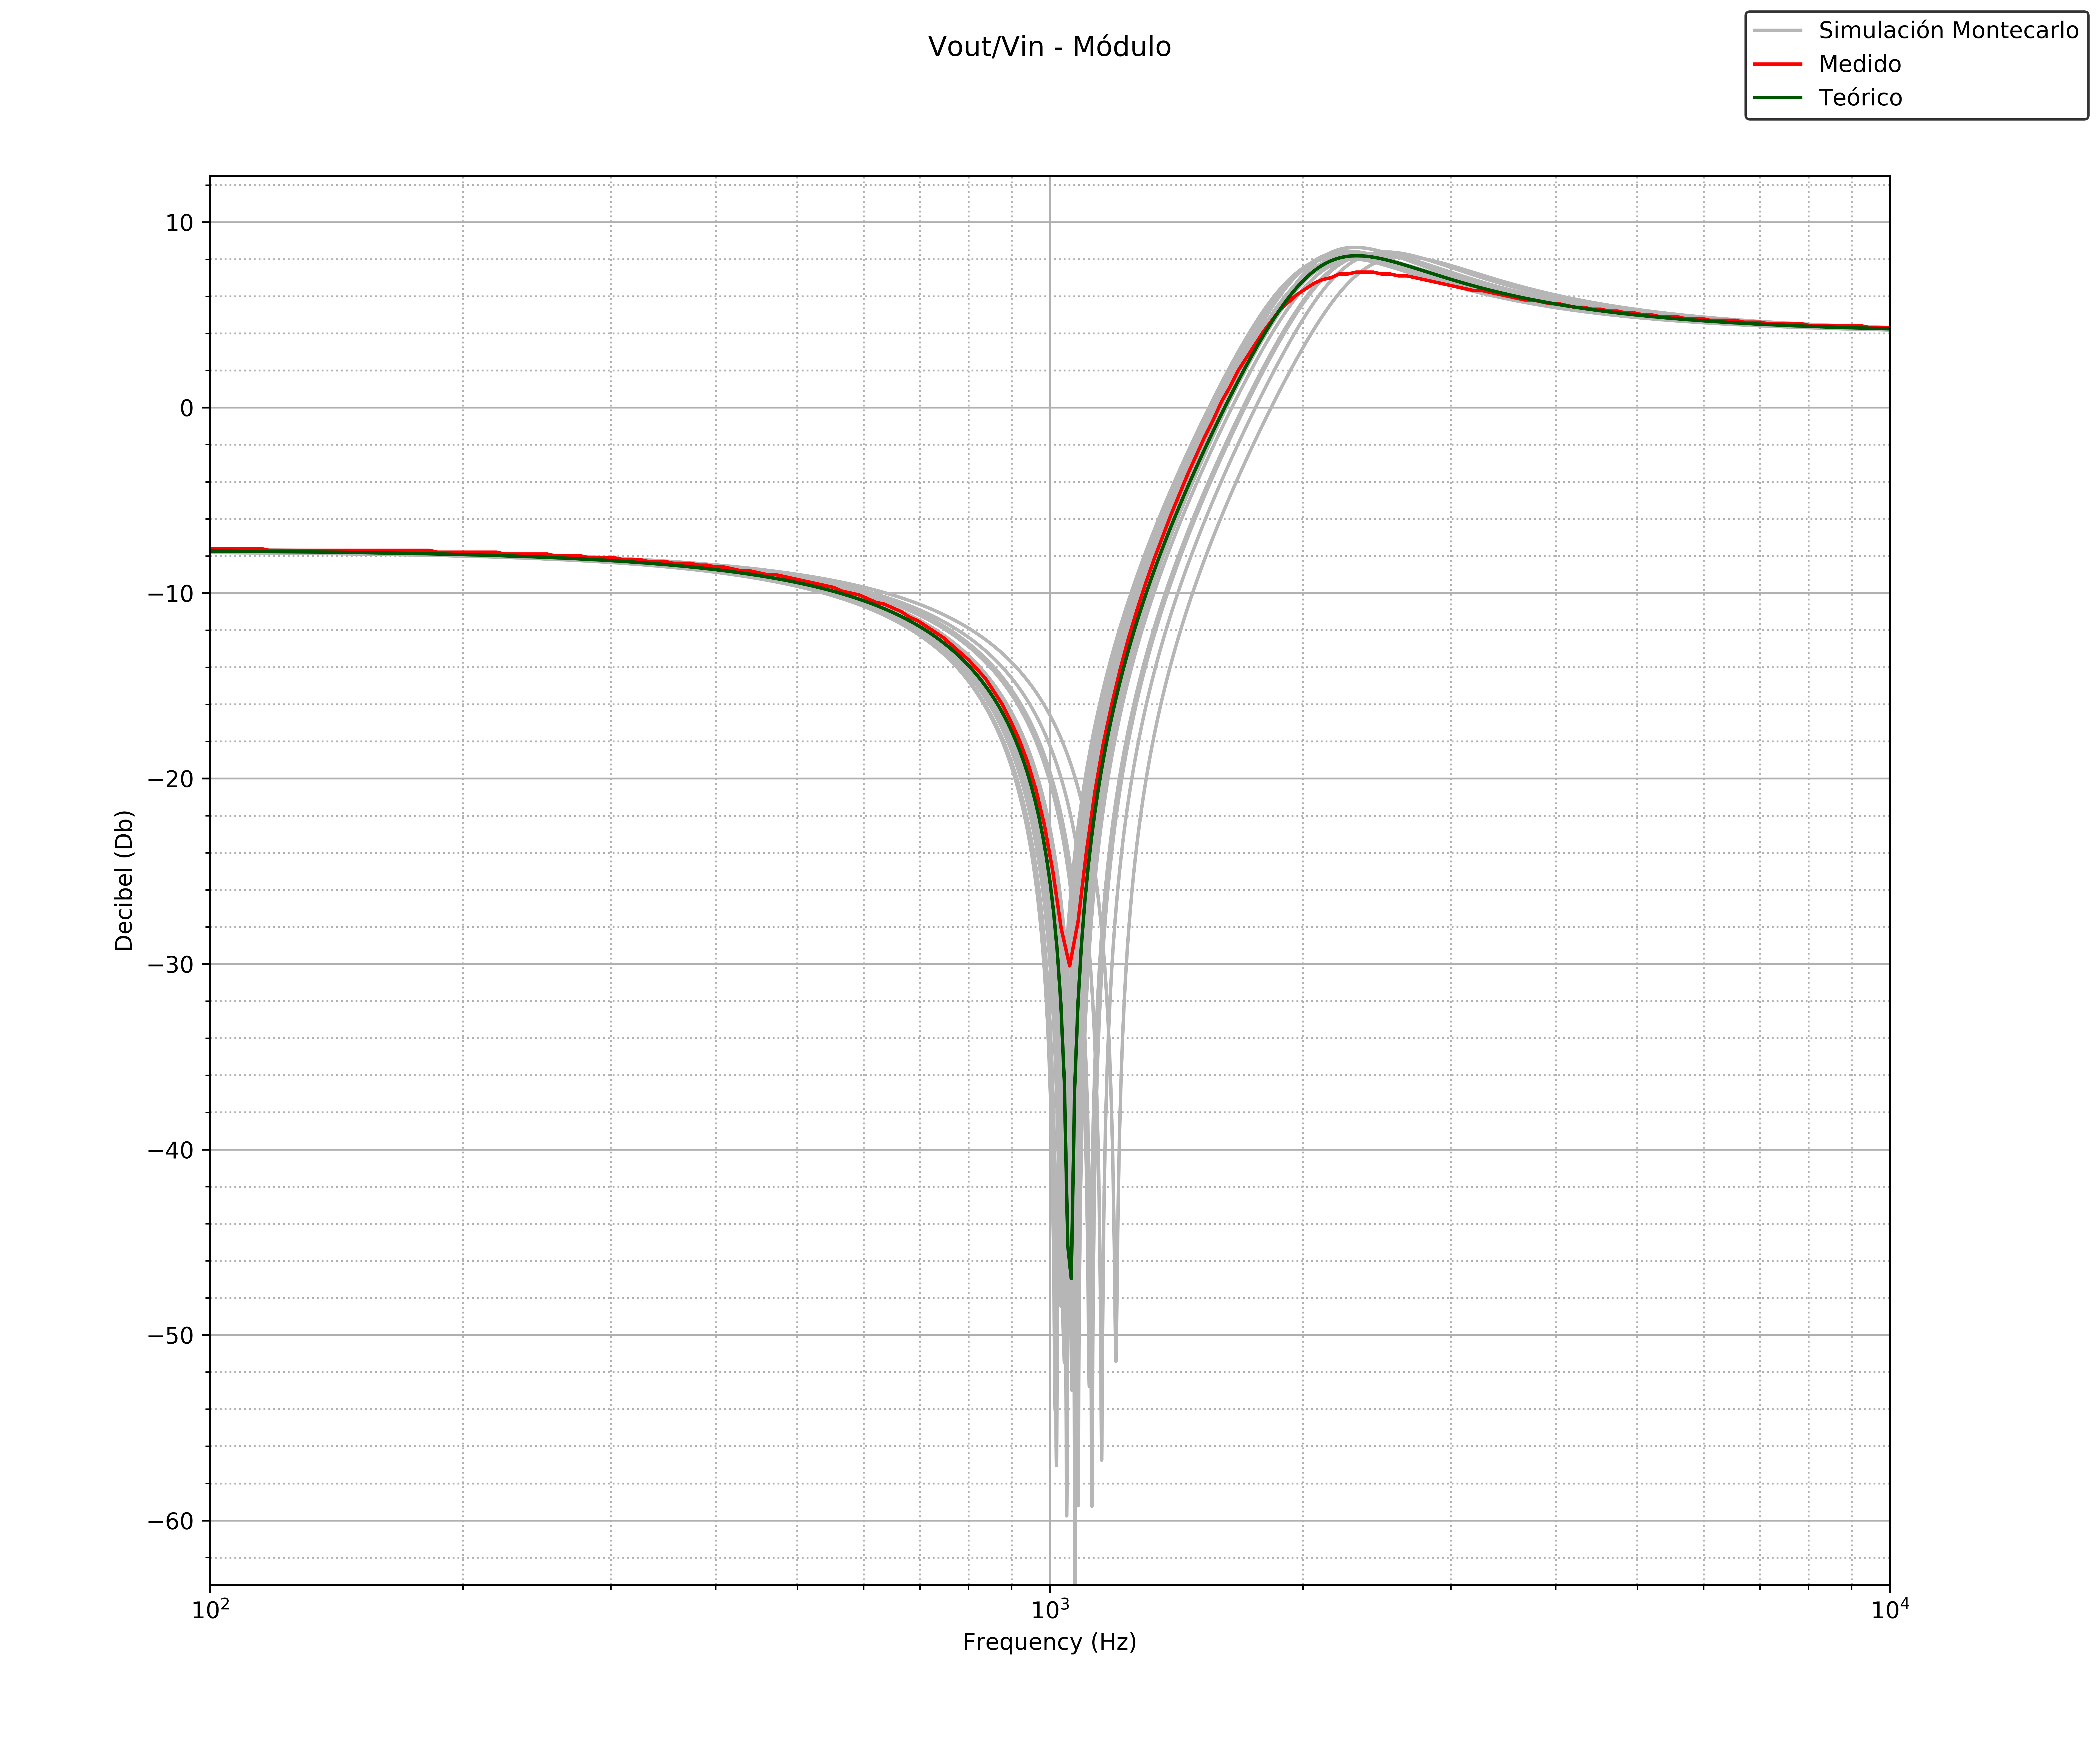
\includegraphics[width=10cm,height=10cm,keepaspectratio]{../EJ1/00GRAFICOS/vovi.png}
	\caption{M\'odulo de la transferencia del circuito.}
	\label{vovi_mod}
\end{figure}

\begin{figure}[H] %!ht
	\centering
	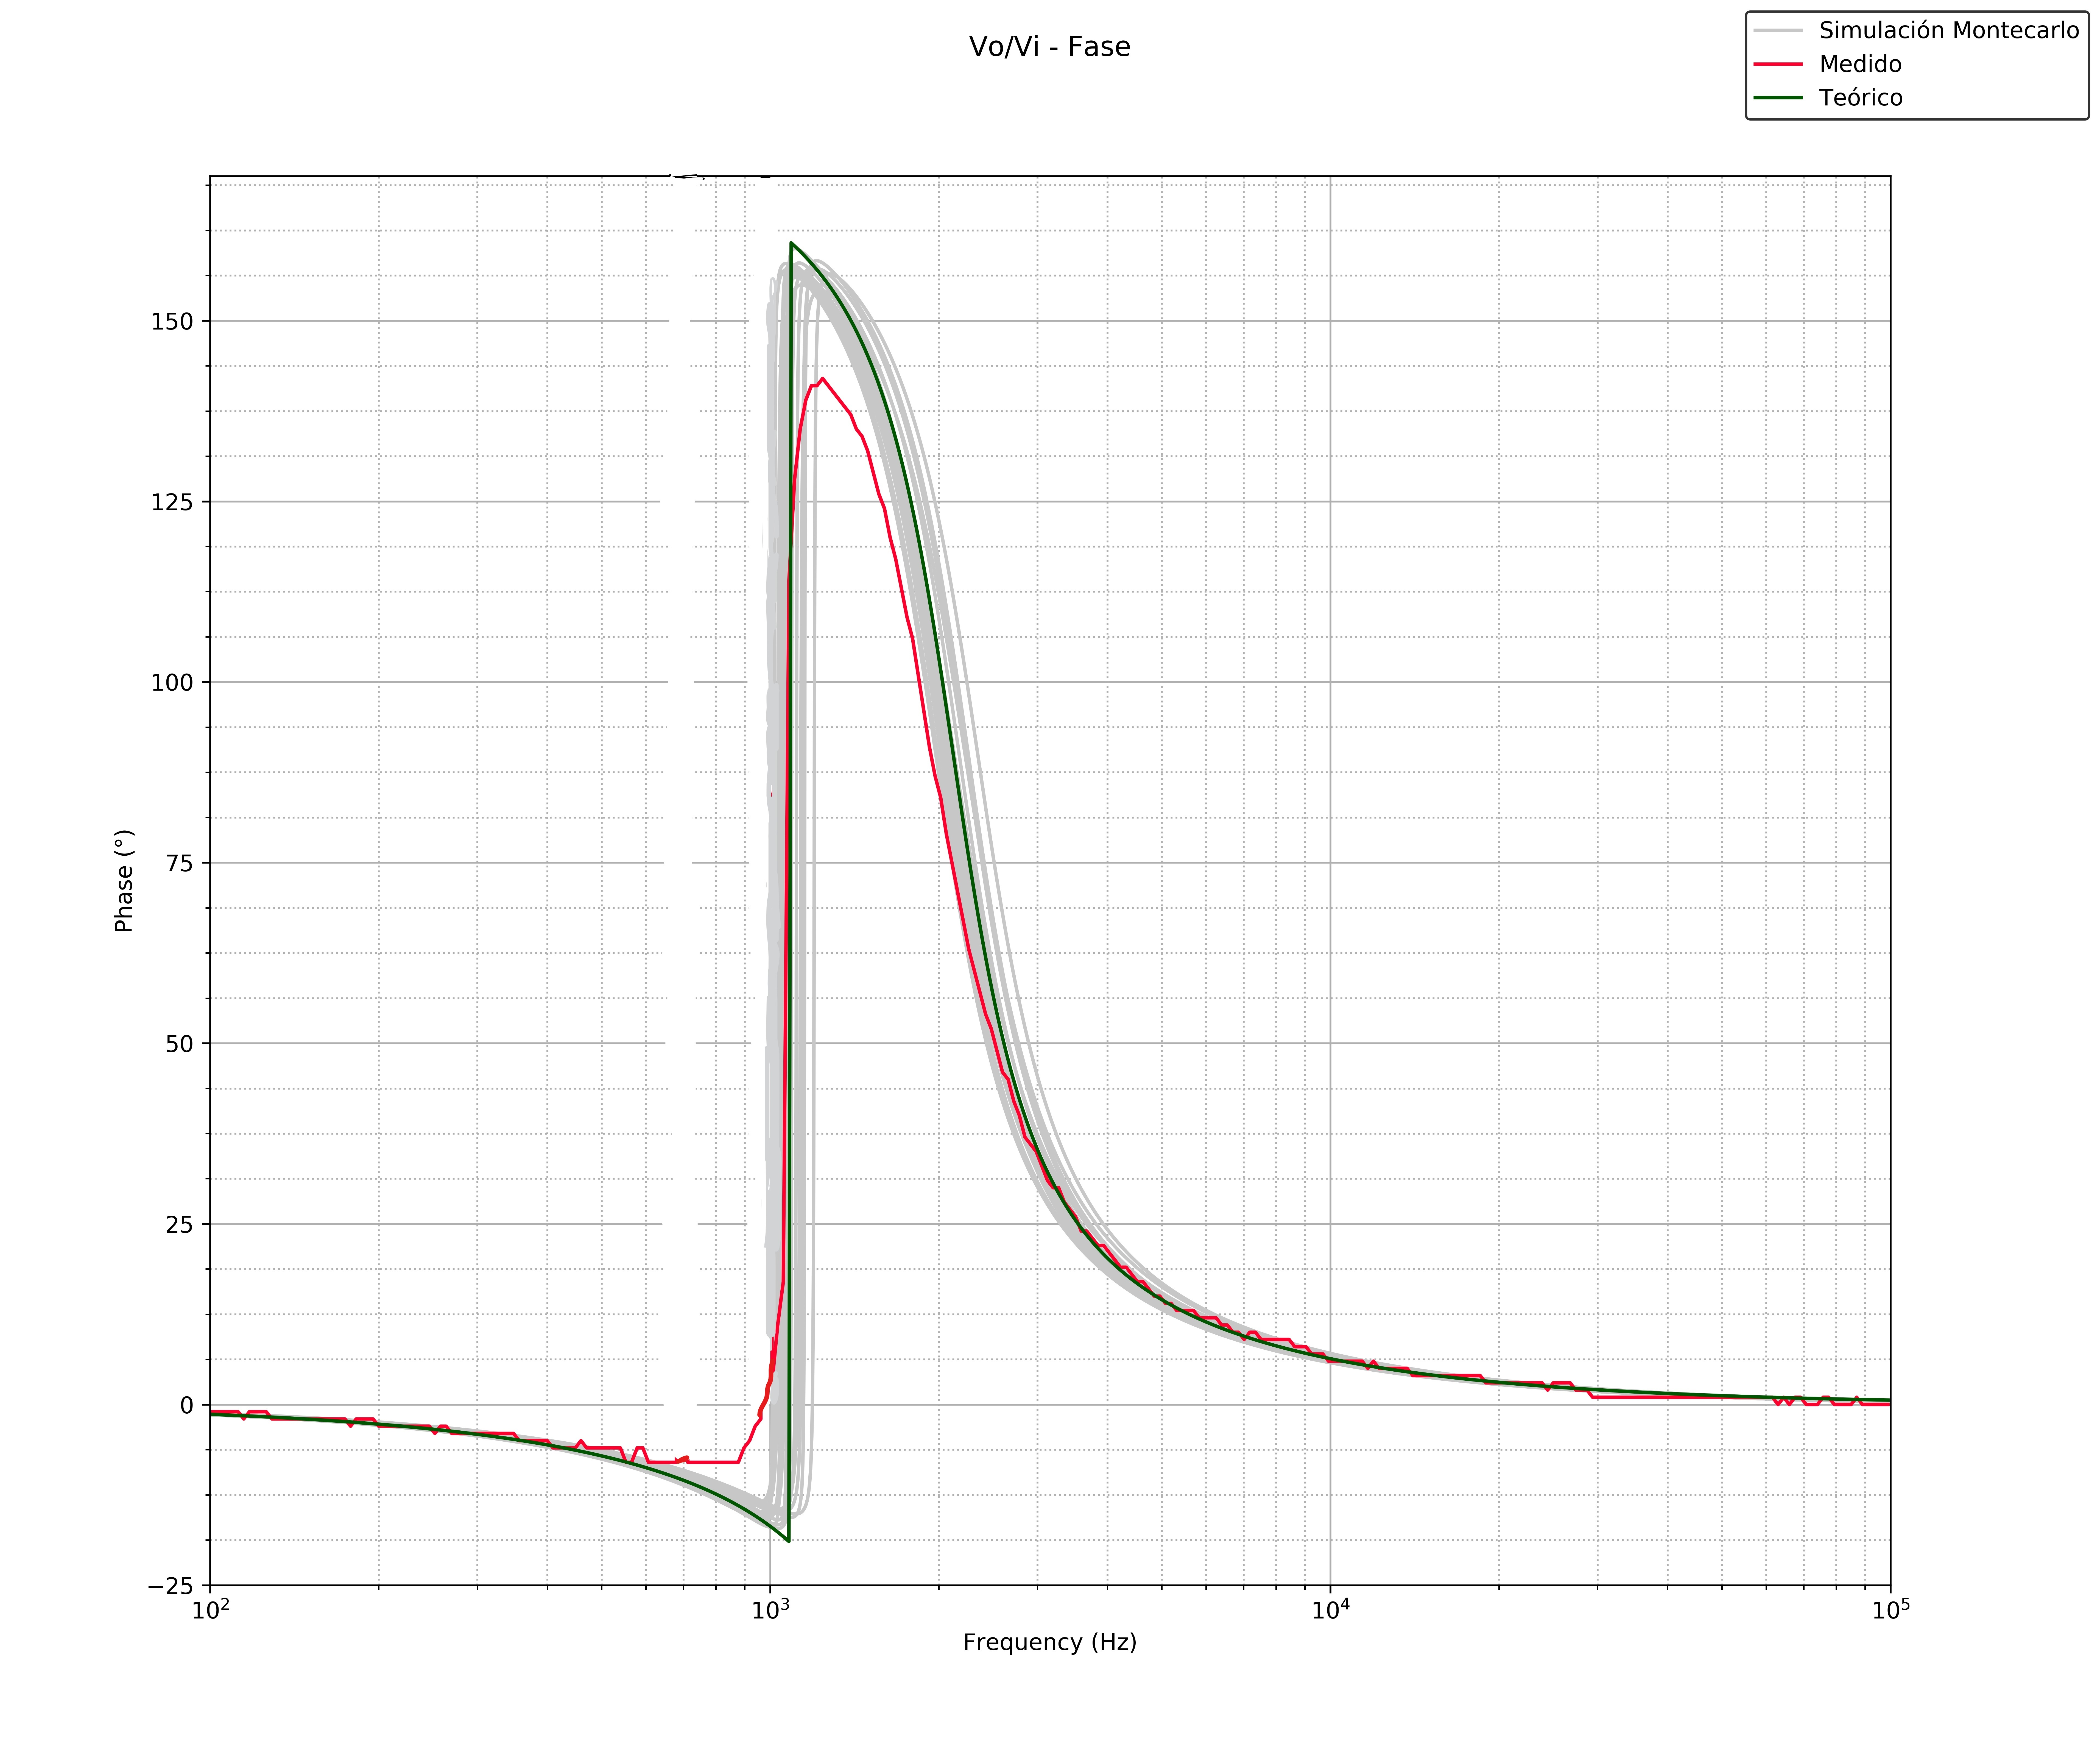
\includegraphics[width=10cm,height=10cm,keepaspectratio]{../EJ1/00GRAFICOS/vovifase.jpg}
	\caption{Fase de la transferencia del circuito.}
	\label{vovi_fase}
\end{figure}

\subsubsection{Impedancia de entrada}

\todo{calcular teoricamente y agregarlo al grafico}
\begin{figure}[H] %!ht
	\centering
	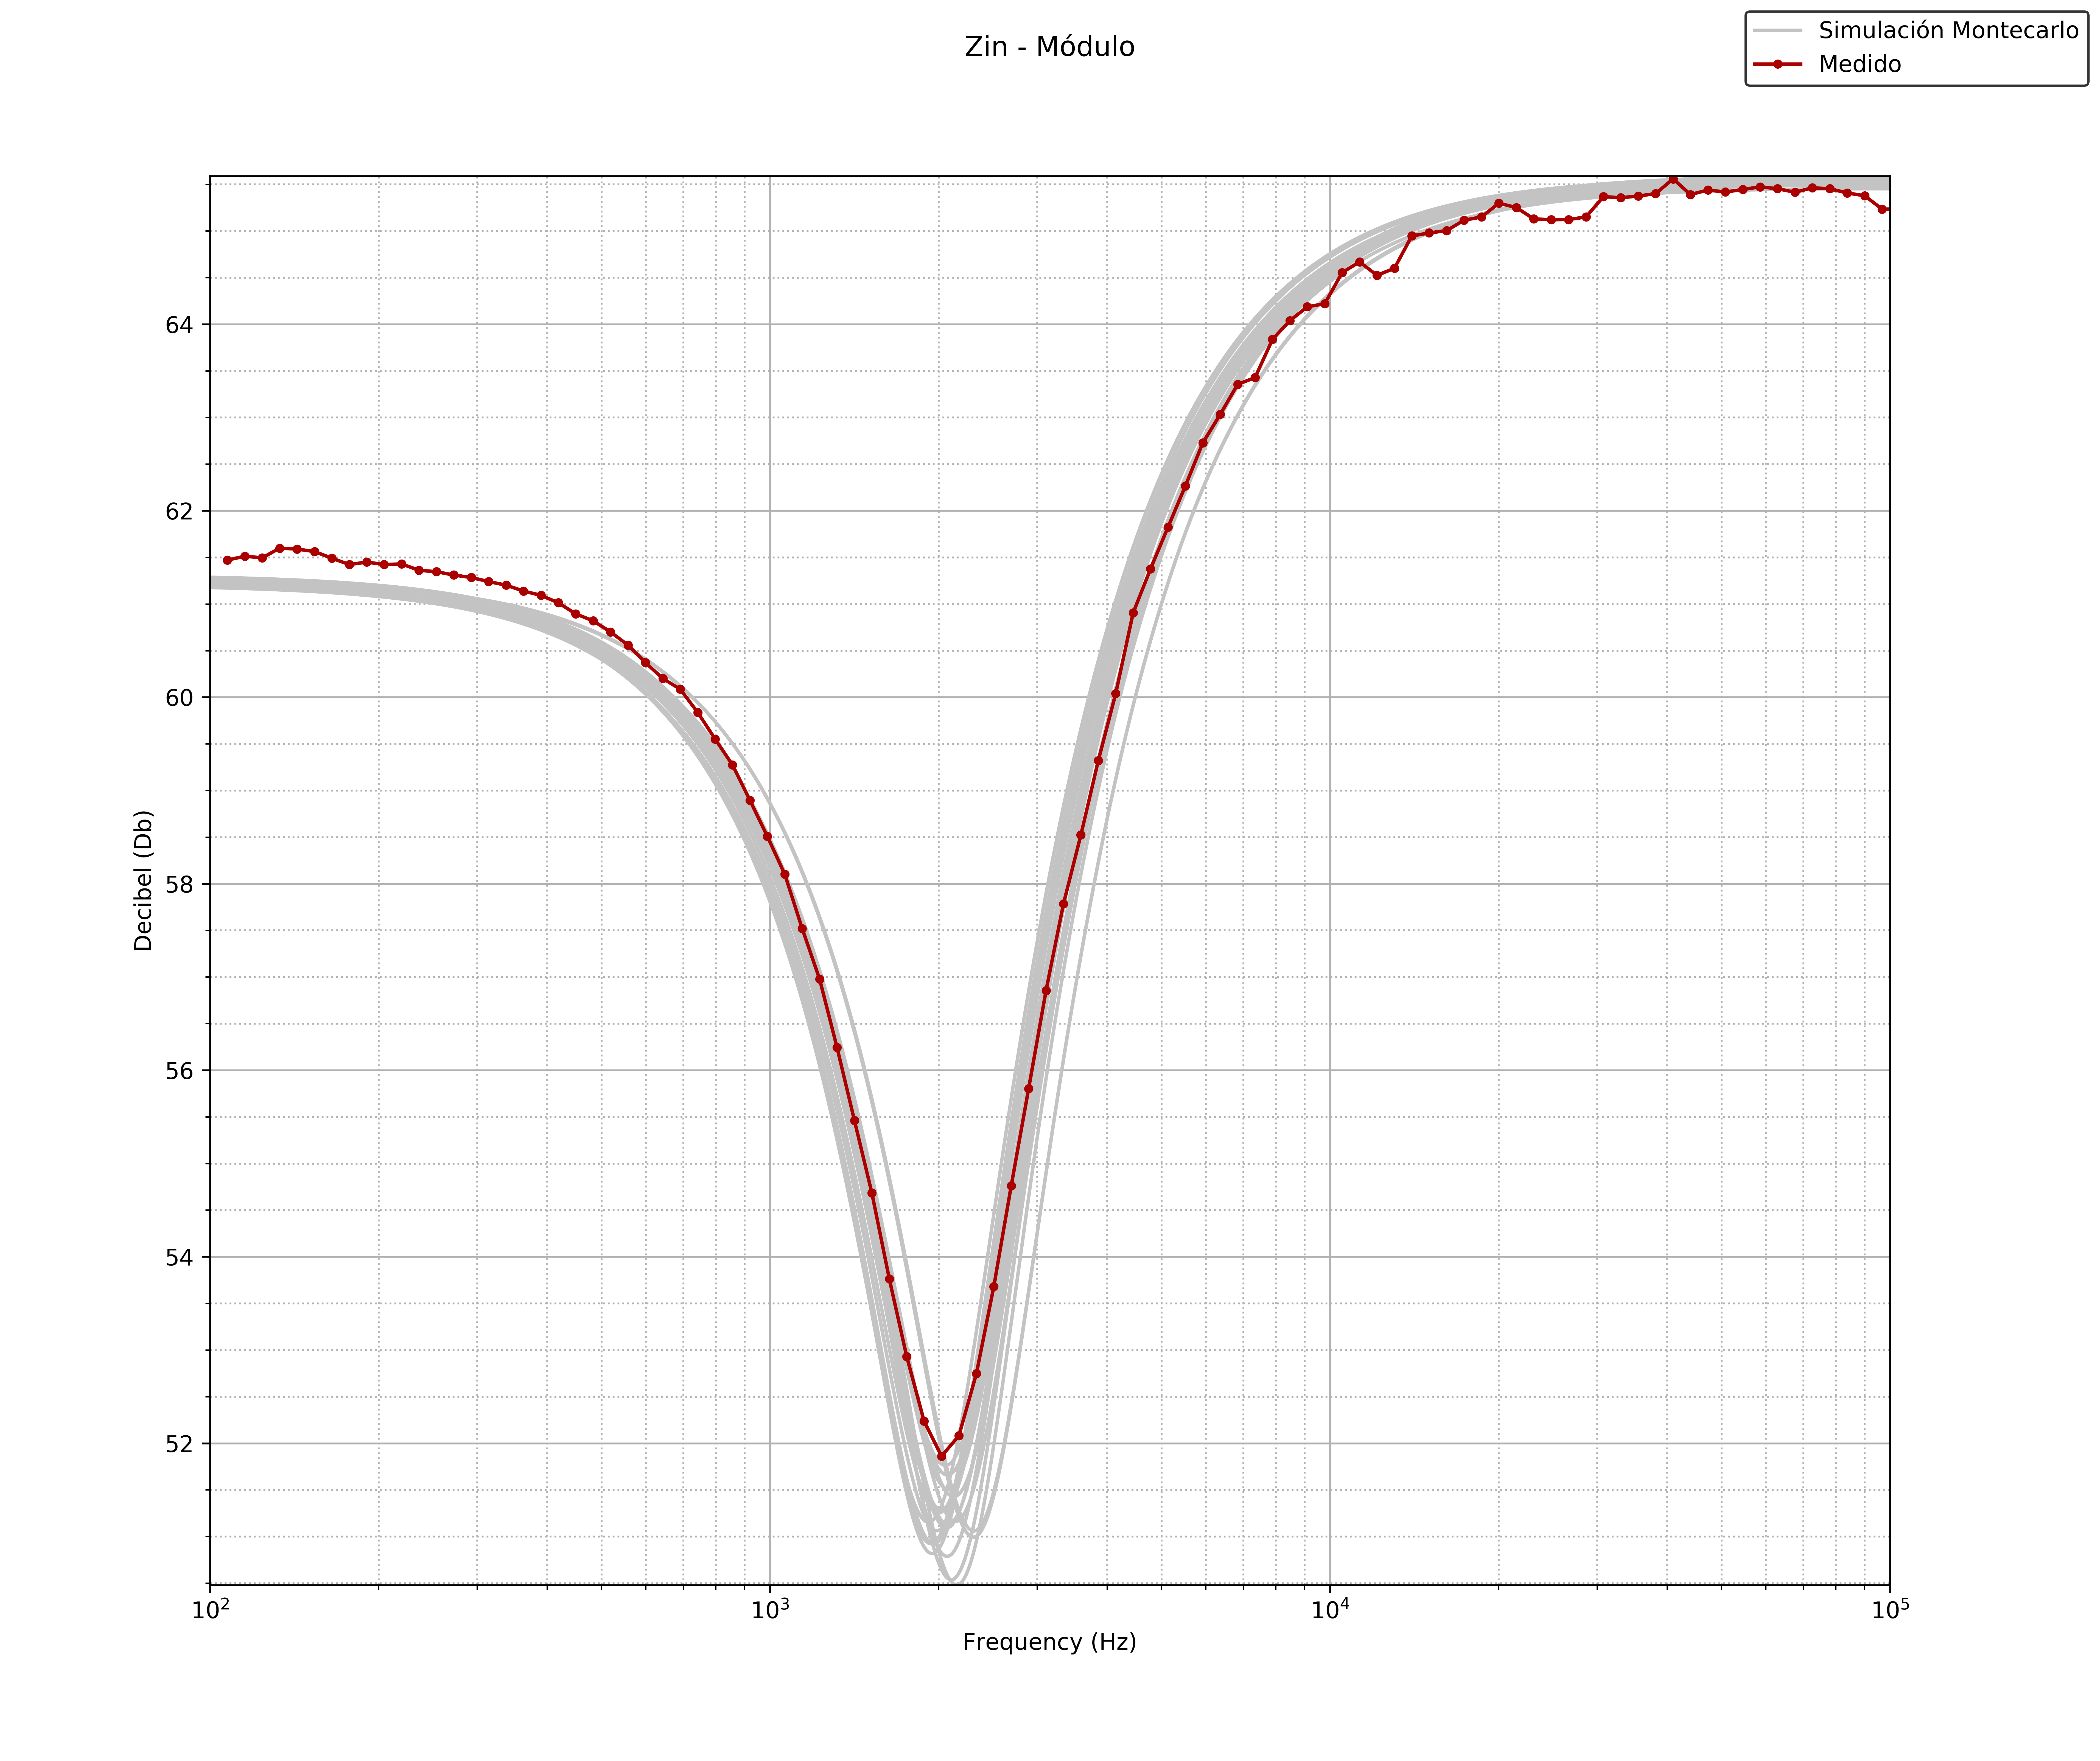
\includegraphics[width=10cm,height=10cm,keepaspectratio]{../EJ1/00GRAFICOS/zin_modulo_sinTeorico.png}
	\caption{Impedancia de entrada.}
	\label{c1vinmax}
\end{figure}

\subsubsection{Impedancia de salida}